\documentclass{article}

\usepackage{cite}
\usepackage[square, comma, numbers, sort&compress]{natbib}
\usepackage{wrapfig}
\usepackage[utf8]{inputenc}
\usepackage[T1]{fontenc}
\usepackage{lmodern}
\usepackage{amsfonts}
\usepackage{amsmath}
\usepackage{graphicx}
\usepackage{booktabs}
\usepackage{placeins}
% \usepackage{pdfpages}
\usepackage{caption}
\usepackage{multirow}
\usepackage{hhline}
\usepackage{capt-of}
\usepackage{array}
\usepackage{subcaption}
\usepackage{here}
\usepackage[labelfont=bf, format=plain, font=it]{caption}
\usepackage[english]{babel}


%kein Zeileneinzug
\parindent=0pt

\begin{document}


\section{Interaction of particles with matter}
\graphicspath{{bilder/1-1/}}
	\subsection{Interaction of charged particles}
		When charged particles interact with matter, only the electromagnetic force is of importance. The
following reactions lead to loss of energy of the charged particles:

\begin{itemize}
  \item ionisation of the atoms in the detector
  \item excitation of the atoms in the detector
  \item bremsstrahlung (relevant for electrons/positrons)
  \item \v{C}erenkov radiation
  \item transition radiation
\end{itemize}

\[-\left(\frac{dE}{dx}\right)_{\text{tot}} = -\left(\frac{dE}{dx}\right)_{\text{coll}}
-\left(\frac{dE}{dx}\right)_{\text{rad}} -\left(\frac{dE}{dx}\right)_{\text{pair}}
-\left(\frac{dE}{dx}\right)_{\text{photo}} -\left(\frac{dE}{dx}\right)_{\text{compton}}
-\left(\frac{dE}{dx}\right)_{\text{kal}}\]

As an example, the total loss of energy $-\frac{dE}{dx}$ of muons in copper is shown in fig.
\ref{enenergylossInCopper}. Most of it can be described by the Bethe formula (the derivation is
explained in the next chapter). Different energies of the projectiles leads through different
interaction to loss of energy.

\begin{figure}[H]
	\centering
	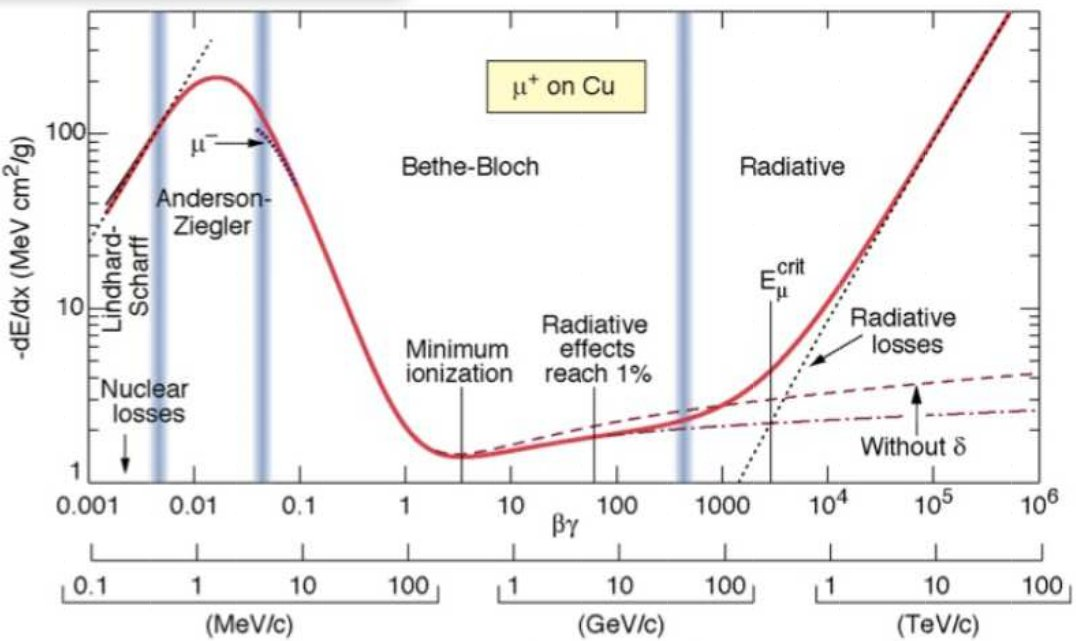
\includegraphics[width=0.5\textwidth]{bethebloch.jpg}
	\caption{Total loss of energy of muons in copper}
	\label{enenergylossInCopper}
\end{figure}

\begin{figure}[H]
	\centering
	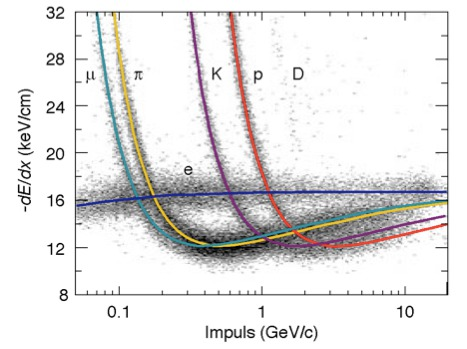
\includegraphics[width=0.5\textwidth]{bethebloch2.jpg}
	\caption{$\frac{dE}{dx}$-Kurven für verschiedene Teilchen (gemessen in der
	PEP4/9-TPC)}
	\label{}
\end{figure}

Notice: $\frac{dE}{dx}$ for heavy particles (e.g. $\alpha$ particles) corresponds well to the Bethe
formula. The energy loss caused by ionisation or excitation of target electrons is dominant.
$\frac{dE}{dx}$ for electrons/positrons, however, do not obey the Bethe formula.
			\subsubsection{Bethe-Bloch-Formel}
				To derive the Bethe formula in a classic way, we consider the energy loss $\frac{dE}{dx}$ of a heavy
(i.e. $m>>m_e$) charged particle scattering on a shell electron of a target atom.
\\
We make the following assumptions:

\begin{itemize}
  \item the shell electron is at rest (neglection of orbital movement and recoil),
  \item the energy transfer is much larger than the binding energy of a shell electron.
\end{itemize}

{\Huge DRAWING}

The momentum transfer is the time integral of the force on the target, caused by the electric field
of the projectile. For the longitudinal and transversal components of the electric field applies

\[E_l(-x)=-E_l(x)~~~~~~~~~~~~~~~~~~~E_t(-x)=E_t(x)\]

i.e. only the transversal component is of importance, as the longitudinal components of the momentum
transfer add up to zero. This yields

\[\Delta p= \int_{-\infty}^{\infty}F\cdot dt = \int_{-\infty}^{\infty}eE_t\cdot dt =
e\int_{-\infty}^{\infty}E_t\frac{dt}{dx}\cdot dx
=e\int_{-\infty}^{\infty}E_t\frac{1}{v}\cdot dx
=\frac{e}{v}\int_{-\infty}^{\infty}E_t\cdot dx\]

With the Gauß formula $\int_{-\infty}^{\infty}E_t2\pi bdx=4\pi ze$ follows

\[\Delta p = \frac{2ze^2}{vb}\]

which yields for the energy transfer

\[\Delta E=\frac{\Delta p^2}{2m_e}=\frac{2z^2e^4}{m_ev^2b^2} .\]

With an electron densitiy of $n_e$, the energy loss results in 

\[-dE(b)=\Delta E(b)n_edv=\frac{2z^2e^4}{m_ev^2b^2}n_e2\pi b db dx\]

After integration from $b_min$ to $b_max$ we obtain:

\[-\left(\frac{dE}{dx}\right)=\frac{4\pi z^2
e^4}{m_ev^2}n_e\text{ln}\left(\frac{b_{\text{max}}}{b_{\text{min}}}\right)\]

Now we have to estimate $b_{\text{min}}$ and $b_{\text{max}}$. $b_{\text{min}}$ we can estimate with
the help of the kinematic limit: A head-on collision yields the greatest possible energy transfer

\[\Delta E_{\text{max}}=\frac{1}{2}m_e(2v)^2\gamma^2.\]

With the obtained relation 

\[\Delta E(b)=\frac{2z^2e^4}{m_ev^2b^2}\overset{!}{=}\Delta E_{\text{max}}\] 

we get

\[b_{\text{min}}=\frac{ze^2}{\gamma m_e v^2}.\]

The estimation of $b_{\text{max}}$ follows from the ``adiabatic invariance'': The target electrons
are bound in atoms and orbit the nucleus with a mean orbital frequency $\overline{\nu}$. The
duration of the disturbance $\Delta t$ has to be shorter than the period $\tau$ for a energy
transfer to happen: 

\[\Delta t=\frac{b}{\gamma v} \le \tau =\frac{1}{\overline{\nu}}\]

This yields 

\[b_{\text{max}}=\frac{\gamma v}{\overline{\nu}}.\]

Now we introduce a quantity for the electron density of the target material:

\[n_e=N_A\cdot \rho\cdot \frac{Z}{A}\]

with the Avogadro number $N_A$, the target density $\rho$, the atomic number $Z$ and mass number
$A$. Inserting the limits for the impact parameter into the formula and substituting $n_e$ leads to 

\[-\left(\frac{dE}{dx}\right)_{\text{coll}} = \frac{4\pi z^2e^4}{m_ev^2}N_A\cdot \rho
\frac{Z}{A}\cdot\text{ln}\left(\frac{\gamma^2 m_e v^3}{2e^2\overline{\nu}}\right), \]

which matches the classical formula of Bohr. This describes the loss of energy of heavy particles
(protons, $\alpha$ particles, \ldots) through excitation and ionisation. For lightweight particles
quantum effects have to be considered.
\\
A quantum mechanical calculation leads to Bethe-Bloch(-Sternheimer) formula:

\[-\left(\frac{dE}{dx}\right)_{\text{coll}} = 2\pi N_A r_e^2 m_e c^2 \rho \frac{Z}{A}
\frac{z^2}{\beta^2}\left[ \text{ln} \left( \frac{2m_e c^2 \gamma^2 \beta^2 W_{\text{max}}}{I^2}
\right) -2\beta^2 -\delta -2\frac{c}{z} \right]\]

with

\[\beta =
\frac{v}{c},~~~~~~~~~~~~\gamma=\frac{1}{\sqrt{1-\beta^2}}~~~~~~~~~~~~
r_e=\frac{1}{4\pi\epsilon_0}\cdot\frac{e^2}{m_e c^2}\]

as well as

sowie
\begin{description}
\item[$z$]charge of the incoming particle
\item[$Z, A$] atomic and mass number of the target
\item[$\rho$] target density
\item[$N_A$] Avogadro number
\item[$I$] mean ionisation potential (material constant of the target)
\item[$W_{\text{max}}$] max. energy transfer in one collision
\item[$\delta$] correction of density (polarisation effects, $\delta \approx 2\text{ln}(\gamma)+K$)
\item[$c$] ``shell correction'' (essential for small velocities of projectiles )
\end{description}

Remarks to Bethe-Bloch formula:

\begin{itemize}
  \item it corresponds well to the loss of energy in the scope of $0,1 < \gamma\beta < 100$;
  \item there are three scopes:
  			\begin{itemize}
  			  \item for low energies, there is a decline down to a minimum (bei $\gamma\beta$
  			  ca. 3-3,5), particles at this point are minimal ionising particles (MIP);
  			  \item after that, a logarithmic incline can be observed for increasing particle energy, the
  			  so-called ``relativistic incline'';
  			  \item for high energies the Fermi plateau is reached: the energy loss approaches a
  			  saturation point caused by polarisation effects (correction of density);
  			  \end{itemize}
  \item the energy loss is a statistical process.
\end{itemize}

The Bethe-Bloch formula describes the mean loss of energy through ionisation and excitation. It
applies to all charged particles except for electrons and positrons. For these, we have to consider
the identic masses and indistinguishability of the collision participants. Our derivation differs
numerically from the Bethe-Bloch formula in a factor of 2, which is caused by a lack of
consideration of distant collisions. There are different variations in the formula of the quantum
mechanical description of the loss of energy $\frac{dE}{dx}$. This is a result of different 
parameterisation of distant collisions, i.e. a loss of energy in which the bond of electrons in the
atomic shell is non-negligible.
\\
Usually, the loss of energy per distance $\frac{1}{\rho}\frac{dE}{dx}$ is given where $\rho$ is the
density in $\frac{\text{g}}{\text{cm}^3}$. $\frac{1}{\rho}\frac{dE}{dx}$ for MIPs is only weakly
dependant of the absorber material und amounts to ca.

\[2 \text{MeV}\frac{\text{cm}^2}{\text{g}}.\]
			\subsubsection{Landau distribution}
				How can the distribution of energy of energy loss be described? The loss of energy is an statistical
process with an asymmetric distribution function, as collisions with small energy transfer is more
probable than those with large energy transfer.

\begin{figure}[H]
	\centering
	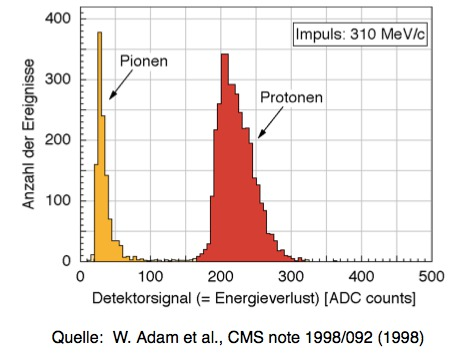
\includegraphics[width=0.5\textwidth]{landau.jpg}
	\caption{Die Energieverteilung des Energieverlustes ist eine Landau-Verteilung.}
	\label{}
\end{figure}

Rarely occuring collisions with small impact parameters lead to tails at high energy transfers. In
this collisions so-called $\delta$-electrons with high energies (keV) are set free. For the mean
loss of energy is higher than the most probable loss of energy, the distribution is asymmetric.
\\
The loss of energy in thin absorbers can be described by a Landau distribution, for thick absorbers,
this merges to a Gaussian distribution.
			\subsubsection{Bragg curve}
				How deep do particles penetrate the detector material? For every combination of projectile and
target, we can only \ldots a mean depth of penetration. The loss of energy of a particle in
dependence of the penetration depth can be described by the Bragg curve. The projectile slows down
when penetrating into matter and the loss of energy increases (Bethe-Bloch). We obtain the range $R$
by integrating  the loss of enegy over the distance, where $\frac{dE}{dx}$ is a function of $E$. For
ionising radiation there is a particular high density of deposited energy  at the end of the range
because of $\frac{1}{\beta^2}$ (dependence).

\[dE= \frac{dE}{dx}(E)dx~~~~~~~~~~\Rightarrow~~~~~~~~~~dx
=\frac{dE}{dE/dx}~~~~~~~~~~\Rightarrow~~~~~~~~~~ R=\int_{E_c}^{M} \frac{dE}{dE/dx}  \]

The highest loss of energy is occurs at the end of the track (Bragg peak).

\begin{figure}[htbp]
	\begin{minipage}[b]{0.5\textwidth}
		\begin{figure}[H]
		\centering
		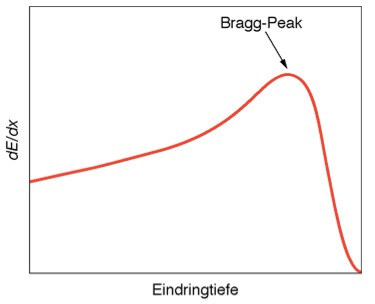
\includegraphics[width=\textwidth]{bragg.jpg}
		\end{figure}
	\end{minipage}
	\hfill
	\begin{minipage}[b]{0.5\textwidth}
		\begin{figure}[H]
		\centering
		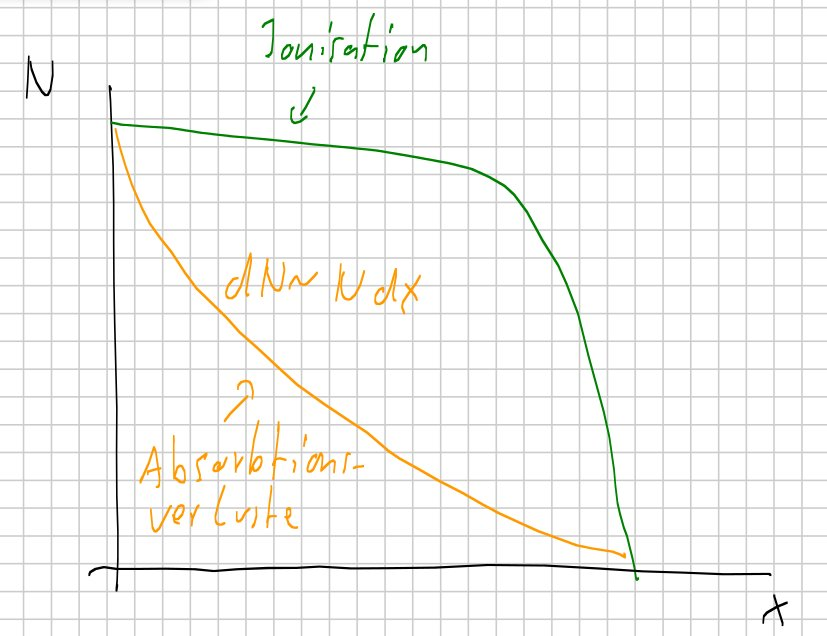
\includegraphics[width=\textwidth]{expabfall.jpg}
		\end{figure}
	\end{minipage}
	\caption{b}
	\label{rekristall} 
\end{figure}
			\subsubsection{Delta electrons}
				The kinetic energy of the electrons is proportional to $\frac{1}{\Delta E^2}$. $\Delta E$ is the
energy transfer of the projectile to the shell electron.

\[\frac{d\sigma}{d\Delta E} = \frac{2\pi z^2 \alpha^2 \hbar^2}{\beta^2 m_e}\cdot \frac{1}{\Delta
E^2}
\]

The tails of this distribution stretch to $\Delta E_\text{max}$,

\[\Delta E_\text{max} = \frac{2m_e c^2 \beta^2 \gamma^2}{1+ 2\gamma
\frac{m_e}{M}+\left( \frac{m_e}{M} \right)^2}\]

with the limits

\begin{itemize}
  \item $\gamma\rightarrow\infty$: $\Delta E \rightarrow \gamma Mc^2$
  \item $m_e \rightarrow M$: $\Delta E \rightarrow m_e c^2 (\gamma -1) = E- m c^2$ \\
  		The entire energy is transfered to the shell electron.
\end{itemize}

These tails can stretch very far for relativistic particles and produce electrons with energies of
several keV. They can be detected as so-called Delta electrons in detectors with high granularity
and spatial resolution.
\\
Rare irradation with high energy leads to more flucuations in $\frac{dE}{dx}$ measurements used to
identify particles and therefore worsens the resolution. Even with detectos of low granularity
does this emission of Delta electrons result in a diminishment of spatial resolution. 
\\
A precise calculation shows:

\[\Delta E (\Theta) = \frac{2m_e}{\text{tan}^2\Theta} \]

Larger angles of irradiation leads to lower energies of the Delta electrons which results in a
shorter range.
			\subsubsection{Energy loss of electrons and positrons}
				Electrons and positrons pose a special case due to their low mass ($m_{e^{\pm}} \approx
511$~keV/c$^2$, $m_{\mu} \approx 106$~MeV/c$^2$). In addition to loss of energy through ionisation
and excitation, the loss of energy through bremsstrahlung gain in importance:

\[-\left(\frac{dE}{dx}\right)_{\text{tot}} = -\left(\frac{dE}{dx}\right)_{\text{coll}}
-\left(\frac{dE}{dx}\right)_{\text{rad}} \]

The Bethe-Bloch formula has to be modified in the case of energy loss through ionisation and
excitation. The loss of energy through ionisation increase logarithmically with $E$ and linearly
with $Z$, whereas the energy loss through bremsstrahlung increases linearly with $E$ and to the
square of $Z$. For high energies (> 1~GeV), bremsstrahlung is the dominating process. 

\begin{figure}[H]
	\centering
	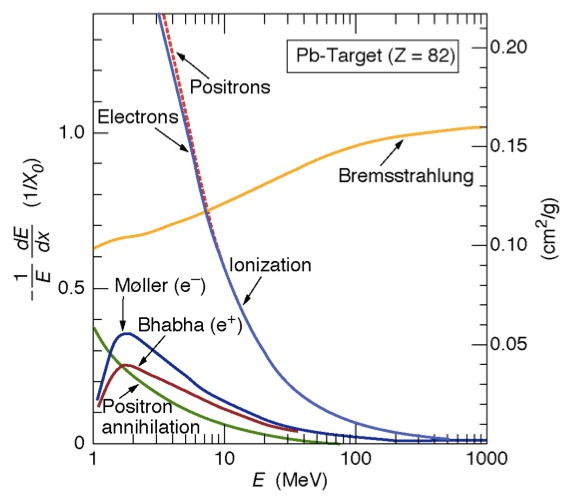
\includegraphics[width=0.5\textwidth]{energieverlust.jpg}
	\caption{}
	\label{}
\end{figure}

			\subsubsection{Bremsstrahlung}
				Bremsstrahlung is emitted, if (high-energetic) charged particles are deflected in an external
electric field, for example the Coulomb field of an atomic nucleus or an shell electron of the
target.
\\
The according Feynman diagrams of lowest order are:
\\
\\
\\
Feynman-Diagramme

\subsubsection*{Energy loss through bremsstrahlung}

For high energies, the loss of energy through bremsstrahlung can be approximated with

\[-\left(\frac{dE}{dx}\right)_{\text{rad}} = 4\alpha \rho N_A \cdot \frac{Z(Z+1)}{A} \cdot z^2\cdot
\left(\frac{1}{4\pi \epsilon_0} \frac{e^2}{mc^2} \right)^2 \cdot E\cdot \text{ln}(183\cdot
Z^{-\frac{1}{3}}) \]

The contribution $Z^2$ is a result of the deflection in the field of the nucleus with the charge
$Z\cdot e$, the one with $Z$ is caused by the deflection in the field of the shell electrons, each
with a charge of $-e$. This does not include that the shell electrons partially shield the nucleus.
Therefore, the formula is only valid for large $E$.
\\
Note: For the second most leightweight particle, the muon, is the loss of energy through
bremsstrahlung already 40,000 times smaller than for the electron.

\[-\left(\frac{dE}{dx}\right)_{\text{rad}} \sim E~~~~~~~~~~\text{und}~~~~~~~~~
-\left(\frac{dE}{dx}\right)_{\text{rad}} \sim \frac{1}{m^2}\]

\subsubsection*{Critical energy $E_c$}

The critical energy is the energy of a projektile where the loss of energy through bremsstrahlung
is equal the loss of energy through the collision:

\[-\left(\frac{dE}{dx}\right)_{\text{rad}} \bigg|_{E_c} = -\left(\frac{dE}{dx}\right)_{\text{coll}}
\bigg|_{E_c}  \]

$E_c$ is dependant of the target material and of the particle type of the projectile (if not
stated otherwise, literature values relate to electrons). The critical energy resizes with about the
square of the mass of the projectile. To obtain the critical energy for muons, for example, we use

\[E_c^\mu = E_c^e \left( \frac{m_\mu}{m_e} \right)^2 \]

There exist different approximations to estimate $E_c$ roughly:

\[E_c = \frac{800}{Z+1{},2}~\text{MeV} \]

or for solids

\[E_c = \frac{610}{Z+1{,}24}~\text{MeV} \]

or for gases

\[E_c = \frac{710}{Z+0{,}92}~\text{MeV} \]

The common values for $E_c$ vary enormously:

\begin{figure}[H]
	\centering
	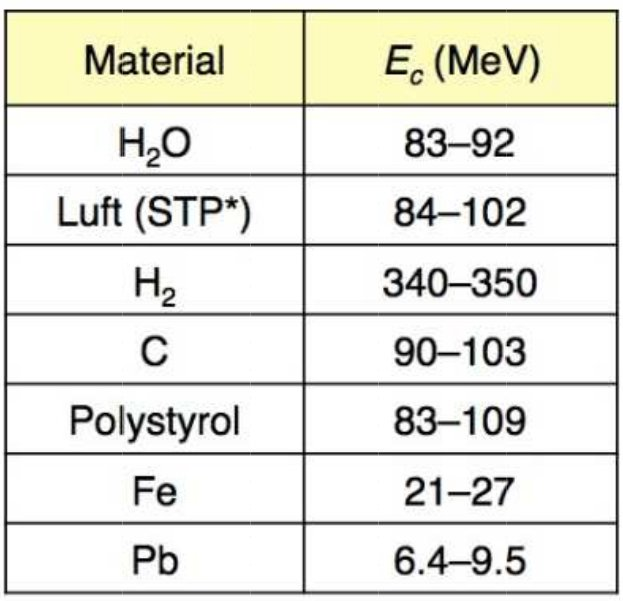
\includegraphics[width=0.5\textwidth]{tabelle1.jpg}
	\caption{}
	\label{}
\end{figure}


\subsubsection*{Radiation length $\chi_0$}



\section{Gas Detectors}
\graphicspath{{bilder/3-1/}}
The relevant processes for loss of energy in gas detectors are excitation and ionisation. 
\\
The excitation of an atom $A$ through a charged particle $x$ via

\[x+A \longrightarrow x+ A^*\]

needs an exact amount of energy in the transfer. Typical cross sections are in the scope of
$\sigma_{\text{Anregung}}=10^{-17}\text{cm}^2$. The excitation energy can be emitted through the
following processes:

\begin{itemize}
  \item Radiation:\\ $A^*\longrightarrow A+h\nu$
  \item Collision:\\ z.B. $\text{Ne}^*+\text{Ar}\longrightarrow \text{Ne}+\text{Ar}^++e^-$
  \item Ion-molecule forming (noble gases):\\ $\text{He}+\text{He} \longrightarrow\text{He}^+_2+e^-$
\end{itemize}

The ionisation of an atom $A$ via

\[x+A \longrightarrow x+ A^+ +e^- \]

however, does not need an exact amount of energy. Typical cross sections are in the scope of
$\sigma_{\text{Ion}}=10^{-16}\text{cm}^2$, which is larger than $\sigma_{\text{Anregung}}$. But as a
large amount of energy is necessary to ionise an atom while transfers with smaller energy are more
frequent, excitation dominates over ionisation.
\\
There are two kinds of ionisation: 

\begin{itemize}
  \item primary ionisation:\\ $x+A \longrightarrow x+A^++e^-$
  \item secondary ionisation:\\ $x+A \longrightarrow x+A^++\delta_{e^-}$ \\ $\delta_{e^-}+A
  \longrightarrow x+A^++e^-$
\end{itemize}

 
	\subsection{Number of electron ion pairs}
		For excitation dominates ionisation, the loss of energy that is necessary to ionise an atom is
larger than the ionisation energy of the atom. The mean number of electron-ion-pairs is given by 

\[\frac{\text{Energieverlust des Teilchens}}{\text{mittlere Energie für die Erzeugung eines
$e^-$-Ion-Paares}} \]

Typical values for the required energy are about $30\,$eV. This way, a particle with $3\,$keV
produces about $\frac{3000\,\text{eV}}{30\,\text{eV}}=100$ $e^-$-ion-pairs.

\begin{figure}[H]
	\centering
	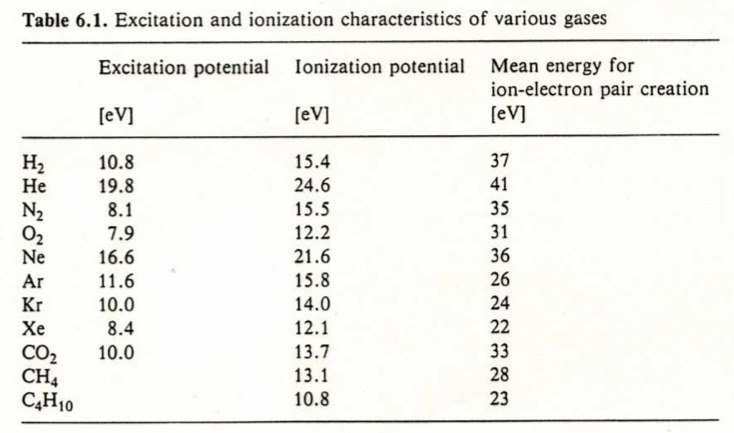
\includegraphics[width=0.5\textwidth]{Fig-03-01.jpg}
\end{figure}

The goal is to determine the loss of energy of particles. The idea is to count the number of the
produced $e^-$-ion-pairs - the larger the number, the more precise the measurement. 

\[\text{particle energy}\approx \#(\text{$e^-$-ion-pairs})\cdot (\text{mean energy for one
$e^-$-ion-pair})\]

For a number $N_{\text{Mess}}\ge 20$, we obtain a Gauss curve for repeated measurements of the
produced primary total ionisation.

\begin{figure}[H]
	\centering
	
\includegraphics[width=0.5\textwidth]{dummy.jpg}
\end{figure}

The relative resolution in this case is given by

\[\frac{\sigma_{a}}{\langle a \rangle} =
\frac{\sqrt{N_{\text{Mess}}}}{N_{\text{Mess}}}=\frac{1}{\sqrt{N_{\text{Mess}}}}
\]

as the best possible resolution for a highly statistical process. In fact, we obtain small values
around the so called Fano factor $F$:

\[ F:=\frac{\text{observed resolution}}{\text{expected resolution (from Poisson statistics)}} \]

Examples:

\ldots

The ionisation processes are not statistically independent!
	\subsection{Free charge carriers in gases}
		One important quantitiy for the description of charge carriers in gases is the mobility $\mu$:

\[v_D = \mu\cdot E \cdot \frac{p_0}{p}  \]

with gas pressure $p$ and $p_0\approx 1013\,$mbar. $\mu$ is the factor of proportionality of the
electric field $E$ and the mean velocity $v_D$ of the charge carrier in this electric field, the
drift velocity.
\\
For gas mixtures, we get

\[\frac{1}{\mu_{i^+}} = \sum_{k=1}^n \frac{c_k}{\mu_{i^+_k}}  \]

with $c_k$ as volume concentration of gas $k$ and $\mu_{i^+_k}$ as mobility of the ion of kind $i$
in gas $k$.


\begin{figure}[H]
	\centering
	
\includegraphics[width=0.5\textwidth]{dummy.jpg}
\end{figure}

\begin{figure}[H]
	\centering
	
\includegraphics[width=0.5\textwidth]{dummy.jpg}
\end{figure}

\begin{figure}[H]
	\centering
	
\includegraphics[width=0.5\textwidth]{dummy.jpg}
\end{figure}


% 	\subsection{Freie Ladungsträger in Gasen: Diffusion}
% 		Even without external electric fields, free charge carriers are in motion due to their thermal
energy. This kind of movement is described by a Maxwell distribution. For ions, we have

\[\langle E_{\text{kin}} \rangle = \frac{1}{2} m \langle u^2 \rangle ~~~~~\text{mit}~~~~ \langle u^2
\rangle = \frac{3kT}{m}
\]

We start with a punctiform charge distribution which then transforms into a \ldots

\begin{figure}[H]
	\centering
	
\includegraphics[width=0.5\textwidth]{dummy.jpg}
\end{figure}

This process can be described with 

\[\frac{dN}{N} = \frac{1}{\sqrt{4\pi\cdot D\cdot t}}\, \text{exp}\left(-\frac{x^2}{4D\cdot
t}\right)\,\mathrm{d}x
\]

whereas the width $\sigma_x=\sqrt{2D\cdot t}$ is dependent of the diffusion coefficient $D$. The
faster the particles are, the larger $D$ gets. In particular, $\langle u^2 \rangle \sim
\frac{1}{m}$ increases with decreasing mass of the particle.
\\
The mean free path in the diffusion process is

\[\lambda(E_{\text{kin}}) = \frac{1}{\frac{N_0\cdot\rho}{A}\cdot \sigma(E_{\text{kin}})}, \]

therefore a function of the kinetic energy of the charged particle.
Previously, the width of the Gaussian distribution applied to diffusion in one dimension. In three
dimension, it is

\[\sigma = \sqrt{6D\cdot t} . \]

The diffusion coefficient can be calculated with the help of kinetic gas theory:

\[D=\frac{1}{3} \langle u \rangle \cdot \lambda~~~~~\text{mit}~~~~\langle u \rangle
=\sqrt{\frac{8kT}{\pi m}}\]

as well as $\lambda$ as mean free path of the charge carrier. That way, we obtain the following
explicit dependencies for $D$:

\begin{itemize}
  \item $D\sim 1/\sqrt{m}$
  \item $D\sim \sqrt{T^3}$
  \item $D\sim 1/\rho$
\end{itemize}

Here, $\sigma_0$ is the total cross section of the impact of the charge carrier with a gas molecule.
% 	\subsection{Rekombinatin und Elektronanlagerung}
% 		\input{3-4-RekombinationUndElektronanlagerung}
% 	\subsection{Elektronendrift in elektrischen Feldern}
% 		\input{3-5-ElektrondriftInElektrischenFeldern}
% 	\subsection{Elektronendrift in elektrischen und magnetischen Feldern}
% 		\input{3-6-ElektrondriftInElUMagFeldern}
% 	\subsection{Gasverstärkung}
% 		\input{3-7-Gasverstaerkung}


\end{document}